\documentclass{article}
\usepackage{amssymb,amsmath,amsthm,bm}
\usepackage{graphicx}
\usepackage{subfigure}
\usepackage{multirow}
% \usepackage{wrapfig}
\usepackage[usenames,dvipsnames]{color}
\usepackage{mathrsfs}
\usepackage{enumerate}
\usepackage[bookmarks=true]{hyperref}
\usepackage{bookmark}

\usepackage{amssymb,amsmath,amsthm}
%\newtheorem{mdef}{Definition}
%\newtheorem{theorem}{Theorem}
\newcommand{\eqsplit}[2]{
  \begin{equation}\label{#2}
    \begin{split}
      #1
    \end{split}
  \end{equation}}
\newcommand{\eqnsplit}[1]{
  \begin{eqnarray*}
    #1
  \end{eqnarray*}}
\newcommand{\tran}[1]{
  \tilde{#1}
}
\newcommand{\td}[2]{
  \frac{d #1}{d #2}
}
\newcommand{\pd}[2]{
  \frac{\partial #1}{\partial #2}
}
\newcommand{\ppd}[2]{
  \frac{\partial^2 #1}{\partial #2^2}
}
\newcommand{\pdd}[3]{
  \frac{\partial^2 #1}{\partial #2 \partial #3}
}
\newcommand{\otd}[1]{
  \frac{d}{d #1}
}
\newcommand{\opd}[1]{
  \frac{\partial}{\partial #1}
}
\newcommand{\oppd}[1]{
  \frac{\partial^2}{\partial #1^2}
}
\newcommand{\opdd}[2]{
  \frac{\partial^2}{\partial #1 \partial #2}
}
\newcommand{\ket}[1]{
  |#1\rangle
}
\newcommand{\bra}[1]{
  \langle#1|
}
\newcommand{\inn}[1]{
  \langle#1\rangle
}
\newcommand{\mean}[1]{
  \langle#1\rangle
}
\newcommand{\tr}{
  \text{tr}\,
}
\newcommand{\re}{
  \text{Re}\,
}
\newcommand\im{
  \text{Im}\,
}
\newcommand{\var}{
  \text{var}
}
\newcommand{\arcsinh}{
  \sinh^{-1}
}
\newcommand{\arccosh}{
  \cosh^{-1}
}
\newcommand{\erfc}{
  \text{erfc}
}
\newcommand{\E}{
  \mathbb{E}
}
\renewcommand{\P}{
  \mathbb{P}
}
\newcommand{\I}[1]{
  \mathbf{1}_{\{#1\}}
}
\newcommand{\1}[1]{
  \mathds{1}_{\{#1\}}
}
\newcommand{\diag}{
  \text{diag\,}
}
\newcommand{\M}{
  {\text{max}}
}
\newcommand{\m}{
  {\text{min}}
}
\newcommand{\ph}{
  {\text{arg}\,}
}
\newcommand\erf{
  \text{erf}
}
\renewcommand\vec[1]{
  \mathbf{#1}
}
\newcommand\mtx[1]{
  \mathbf{#1}
}
\newcommand\ed{
  \,{\buildrel d \over =}\,
}



\DeclareGraphicsExtensions{.eps, .pdf}

\author{
  Prof. Sven \AA berg \\
  Xie Xiaolei}
\date{\today}
\title{Effect of Heteroscedasticity in Covariance Matrix}

\begin{document}
\maketitle

\section{Separation of the Heteroscedasticity Effect}
Consider a covariance matrix constructed as
$$
C_{ij} = {1 \over T}\sum_{t=1}^T r_{it} r_{jt}
$$
where $r_{it}$ is the log-return of the $i$-th stock at time $t$. $i =
1, 2, \dots, N$, $t = 1,2,\dots,T$. Here and in the rest of the
text we adopt a stochastic volatility model for $r_{it}$, i.e.
$$
r_{it} = \sigma_{it} \eta_{it}
$$
where $\sigma_{it}$ symbolizes the volatility of the return while
$\eta_{it}$ is assumed a standard normal random variable.
So we can write
\begin{eqnarray}
C_{ij} &=& {1 \over T}\sum_{t=1}^T \sigma_{it} \eta_{it} \sigma_{jt}
\eta_{jt} \nonumber \\
\bm{C} &=& {1 \over T} (\bm{\sigma * \eta}) (\bm{\sigma *
  \eta})' \label{eq:C}
\end{eqnarray}
where the matrices $\bm{\sigma}$ and $\bm{\eta}$ have elements
$\sigma_{it}$ and $\eta_{it}$ respectively, and * denotes element-wise
multiplication. Due to the cyclic property of matrix trace, the
moment generating function of $\bm{C}$, $M_C(z)$, relates to $M_D(z)$,
the moment generating function of
\begin{eqnarray*}
  \bm{D} &=& {1 \over T} (\bm{\sigma * \eta})' (\bm{\sigma * \eta})
\end{eqnarray*}
through the equation
\begin{eqnarray*}
  M_C(z) &=& {1 \over q} M_D(z)
\end{eqnarray*}
where $q = N/T$. For later convenience, we make use of $T \times T$
matrices $\bm{\tilde{\sigma}}$ and $\bm{\tilde{\eta}}$, as well as a
projector
$$
\bm{P} = \text{diag}(\underbrace{1, \cdots, 1}_{\text{N 1's}}, 
\underbrace{0, \cdots, 0}_{\text{T-N 0's}})
$$
The first N rows of $\tilde{\bm{\sigma}}$ and $\bm{\tilde{\eta}}$ are
precisely those of $\bm{\sigma}$ and $\bm{\eta}$. This way, we have
\begin{eqnarray*}
\bm D &=& {1 \over T} (\bm{\sigma * \eta})' (\bm{\sigma * \eta}) \\
&=& {1 \over T} (\bm{\tilde{\sigma} * \tilde{\eta}})' \bm P'
\bm P (\bm{\tilde{\sigma} * \tilde{\eta}}) \\
&=& {1 \over T} (\bm{\tilde{\sigma} * \tilde{\eta}})'
\bm P (\bm{\tilde{\sigma} * \tilde{\eta}}) \\
\end{eqnarray*}
Again, by the cyclic property of matrix trace, the spectral properties
of the RHS of the last equation is equivalent to those of
\begin{eqnarray*}
  \bm E &=& {1 \over T} (\bm{\tilde{\sigma} * \tilde{\eta}}) (\bm{\tilde{\sigma}
    * \tilde{\eta}})' \bm P \\
\end{eqnarray*}
In the simple situation where $\sigma_{it} =
\sigma_{jt} = \sigma_t$ for some $\sigma_t$ and for all $i, j, t$,
\begin{eqnarray*}
  \bm{\tilde \sigma * \tilde \eta} &=& \bm{\tilde \eta}
  \begin{pmatrix}
    \sigma_1 &        & \\
        & \ddots & \\
        &        & \sigma_T
  \end{pmatrix} \\
  &=& \bm{\tilde \eta \bar \sigma}
\end{eqnarray*}
Thus
\begin{eqnarray}\label{eq:E_def}
  \bm E &=& {1 \over T}\bm{\tilde \eta \bar \sigma^2 \tilde \eta' P}
\end{eqnarray}
In the large T limit $\bm{\tilde \eta \bar \sigma^2 \tilde \eta'}$ and $P$ are
freely independent, therefore their S-transforms are multiplicative,
i.e.
\begin{eqnarray}
  S_E(z) &=& S_{\tilde \eta \bar \sigma^2 \tilde \eta'/T}(z) S_P(z)
  \nonumber \\
  &=& S_{\tilde \eta' \tilde \eta /T}(z) S_{\bar \sigma^2}(z) S_P(z) \label{eq:S_E}
\end{eqnarray}
For $S_{\tilde \eta' \tilde \eta /T}(z)$ there have been results when
the elements of $\bm{\tilde \eta}$ are identically distributed with finite
second moment \cite{burda2011} or alternatively, follow a stable
distribution \cite{politi2010}.

So our focus hereafter is on the spectral properties of $\bar{
\bm \sigma^2}$. The Green's function of $\bar{\bm \sigma^2}$
can be immediately written down:
\begin{eqnarray*}
G_{\bar \sigma^2} &=& \frac{1}{T}\sum_{t=1}^T \frac{1}{z - \sigma_t^2}
\end{eqnarray*}
Suppose the $\sigma_t^2$ process has correlation time $\tau$,
i.e. $\text{corr}(\sigma_t^2, \sigma^2_{t+\tau}) \approx 0$. Then we
have
\begin{eqnarray*}
G_{\bar \sigma^2} &=& {1 \over T}\sum_{n=0}^{\tau-1}\sum_{m=1}^{T/\tau}
\frac{1}{z - \sigma_{m\tau + n}^2} \\
&=& {1 \over \tau}\sum_{n=0}^{\tau-1} {1 \over T/\tau}
\sum_{m=1}^{T/\tau} \frac{1}{z - \sigma_{m\tau + n}^2} \\
&=& {1 \over \tau}\sum_{n=0}^{\tau-1}
\E_m\left(\frac{1}{z - \sigma_{m\tau + n}^2}\right)
\end{eqnarray*}
where $\E_m$ denotes averaging over the index $m$. On condition that
$\sigma_t^2$ is a stationary process, $\E_m[1 / (z -
    \sigma_{m\tau + n}^2)]$ is independent of $n$. Thus
\begin{eqnarray}\label{eq:greens}
G_{\bar \sigma^2} &=& \E_m\left(
  \frac{1}{z - \sigma_{m\tau + n}^2}
\right)
\end{eqnarray}
So autocorrelations of $\sigma_t^2$'s affect spectral properties
only through the stationary distribution of $\sigma_t^2$.
In the following subsections we discuss situations where $\sigma_t$'s
are chosen from different conditional distributions and have different
autocorrelation structures.
% Then the moment generating function $M_{\bar \sigma^2}$ is
% \begin{eqnarray*}
%   M_{\bar \sigma^2} &=& z G_{\bar \sigma^2} - 1 \\
%   &=& \frac{1}{T} \sum_{t=1}^T \frac{1}{1 - \sigma_t^2/z} - 1\\
%   &=& \frac{1}{T} \sum_{n=0}^{\infty} \frac{1}{z^n}\sum_{t=1}^T
%   \sigma_t^{2n} - 1\\
%   &=& \frac{1}{T} \sum_{n=1}^{\infty} \frac{1}{z^n}\sum_{t=1}^T
%   \sigma_t^{2n}
% \end{eqnarray*}

\section{Normal innovations \& log-normal volatilities with AR(1)
  autocorrelation}
In this subsection we consider the case
\begin{eqnarray}
  \log \sigma_t &=& \phi\log \sigma_{t-1} + x_t \nonumber \\
  &=& \sum_{l = 0}^{\infty} \phi^l x_{t-l} \label{eq:AR}
\end{eqnarray}
where $x_t \sim N(0, \theta^2)$ and we have assumed that the $\log
\sigma_t$ process was started in the infinite past with $\log
\sigma_{-\infty} = x_{-\infty}$. In addition, we assume $\log
\sigma_t$ is a stationary process with $|\phi| < 1$. Clearly $\log
\sigma_t$ is normally distributed with mean 0 and variance ${\theta^2
  / (1 - \phi^2)}$. According to \eqref{eq:greens}, the spectral
density of $\bm E$ as appears in \eqref{eq:E_def} is the same as if
$\sigma_t^2$'s were uncorrelated but $\log \sigma_t \sim N(0,
\theta^2/(1 - \phi^2))$.

To find the spectral density of $\bm C$ with normally distributed $\bm
\eta$ and uncorrelated, log-normally distributed $\sigma_t$, we use
the result of Biroli et al in \cite{biroli2007student}, which gives
the Blue function of $\bm C$ as
\begin{eqnarray*}
  B(z) &=& \frac{1}{z} + \int \frac{\sigma ^2 P(s) ds}{1-q \sigma ^2 z}
\end{eqnarray*}
where $q = N/T$ and $\sigma$ has the stationary distribution of
$\sigma_t$, whose probability density function is $P(s)$. Now we are
specifically considering lognormally distributed $\sigma_t$, so we
rewrite the above equation as
\begin{eqnarray}
B(z) &=& \int_{-\infty }^{\infty } \frac{e^{2 s} \exp \left(-\frac{s^2}{2
      v}\right)}{\sqrt{2 \pi  v} \left(1-q e^{2 s} z\right)} \,
ds+\frac{1}{z} \label{eq:LognormalBlue}
\end{eqnarray}
where $v = 1/(1 - \phi^2)$, reflecting the effect
of autocorrelation in $\log \sigma_t$'s. However, no closed form of
this integral is known to the author. To obtain the spectral density,
which is given by the Sokhotski-Weierstrass formula as
\begin{eqnarray}
  \rho(\lambda) &=& -{1 \over \pi} \lim_{\epsilon \to 0} \im G(\lambda +
  i\epsilon) \label{eq:Sokhotski-Weierstrass}
\end{eqnarray}
we equate the real part of RHS of \eqref{eq:LognormalBlue} to $\lambda \in
R$ and the imaginery part to 0, then we can solve \eqref{eq:LognormalBlue}
numerically and obtain $\rho(\lambda)$ via
\eqref{eq:Sokhotski-Weierstrass}. Specifically we solve the following
equation system:
\begin{eqnarray}
\lambda &=& \int_{-\infty}^{\infty} \frac{ds}{\sqrt{2\pi v}}
\frac{
  e^{-s^2/2v}(e^{-2s} - qx)
}{
  (e^{-2s} - qx)^2 + q^2 y^2  
} +
\frac{x}{x^2 + y^2} \label{eq:LognormalBlueReal}\\
0 &=& \int_{-\infty}^{\infty} \frac{ds}{\sqrt{2\pi v}}
\frac{
  e^{-s^2/2v} q y
}{
  (e^{-2s} - qx)^2 + q^2 y^2  
} -
\frac{y}{x^2 + y^2} \label{eq:LognormalBlueImag}
\end{eqnarray}
This is the method used by Biroli et al in
\cite{biroli2007student}. Figure \ref{fig:LognormalBlue}
shows the plot of the Blue function \eqref{eq:LognormalBlue}. $-\pi
\rho(\lambda)$ is the projection of the contour $\im B(z) = 0$ onto the $\im
G$ axis.
\begin{figure}[htb!]
  \centering
    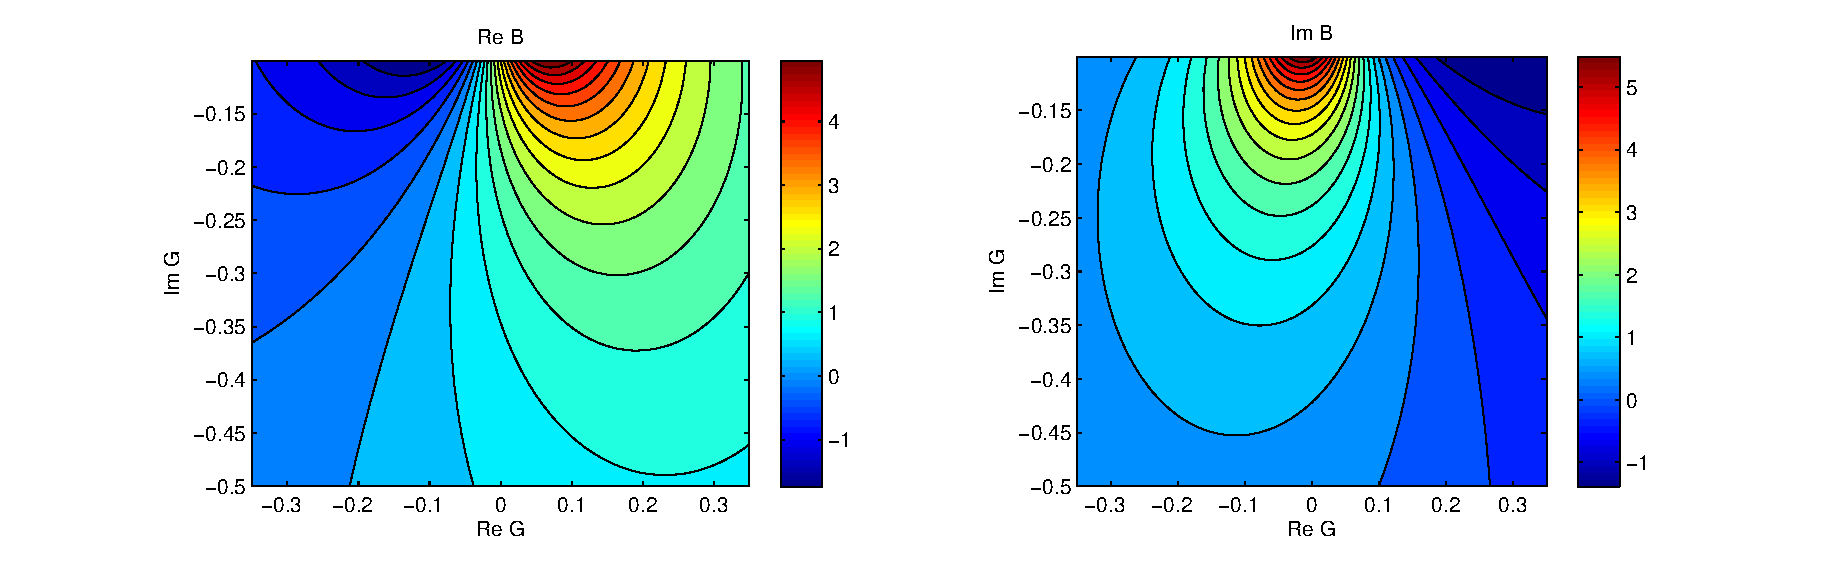
\includegraphics[scale=0.45, clip=true, trim=66 0 84
    0]{../pics/LognormalBlue.eps}
  \caption{\small \it The Blue function $B$. q = 0.45, v = 3}
  \label{fig:LognormalBlue}
\end{figure}
The spectral density function $\rho(\lambda)$ obtained as numerical
solutions is shown in figure \ref{fig:LognormalSpectra} and compared
to the Marcenko-Pastur law with several values of $q = N/T$ and $v$.
\begin{figure}[htb!]
  \centering
  \subfigure[$q = 0.1$]{
    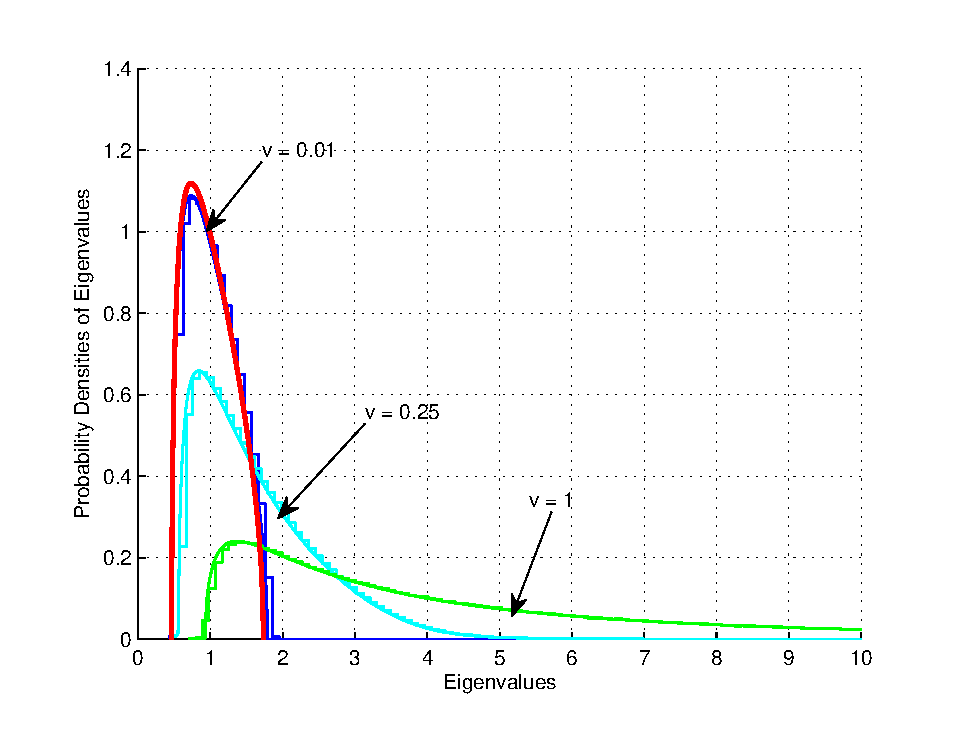
\includegraphics[scale=0.35]{../pics/Lognormal_q0.1.eps}
    \label{fig:Lognormal_q0.1}
  }
  \subfigure[$q = 0.2$]{
    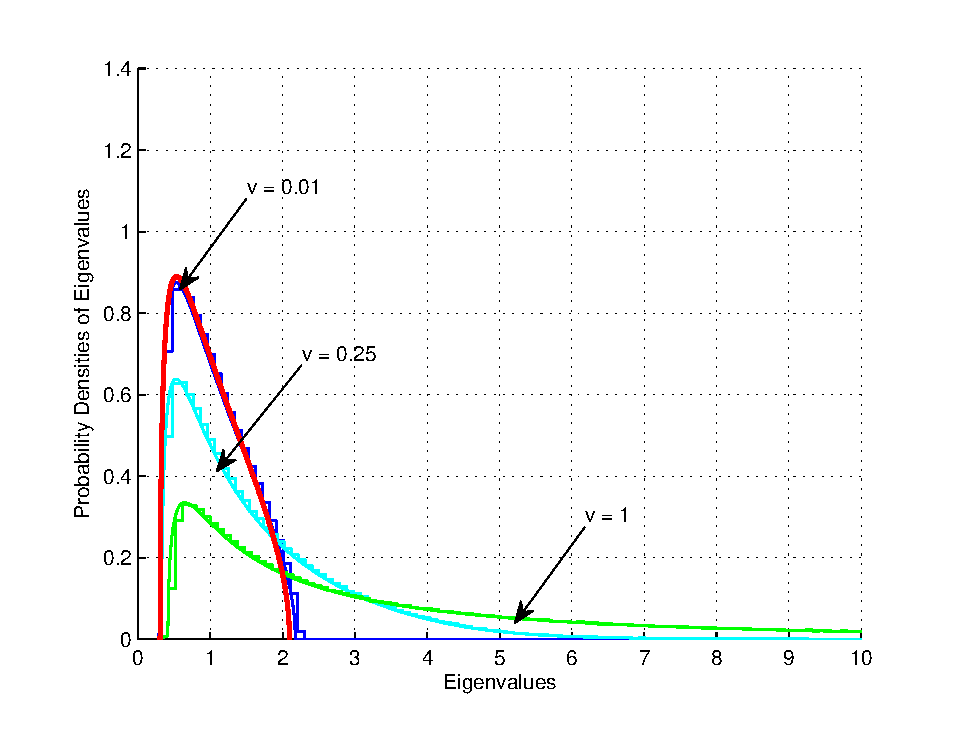
\includegraphics[scale=0.35]{../pics/Lognormal_q0.2.eps}
    \label{fig:Lognormal_q0.2}
  }
  \subfigure[$q = 0.5$]{
    \includegraphics[scale=0.35]{../pics/Lognormal_q0.5.eps}
    \label{fig:Lognormal_q0.5}
  }
  \subfigure[$q = 1.0$]{
    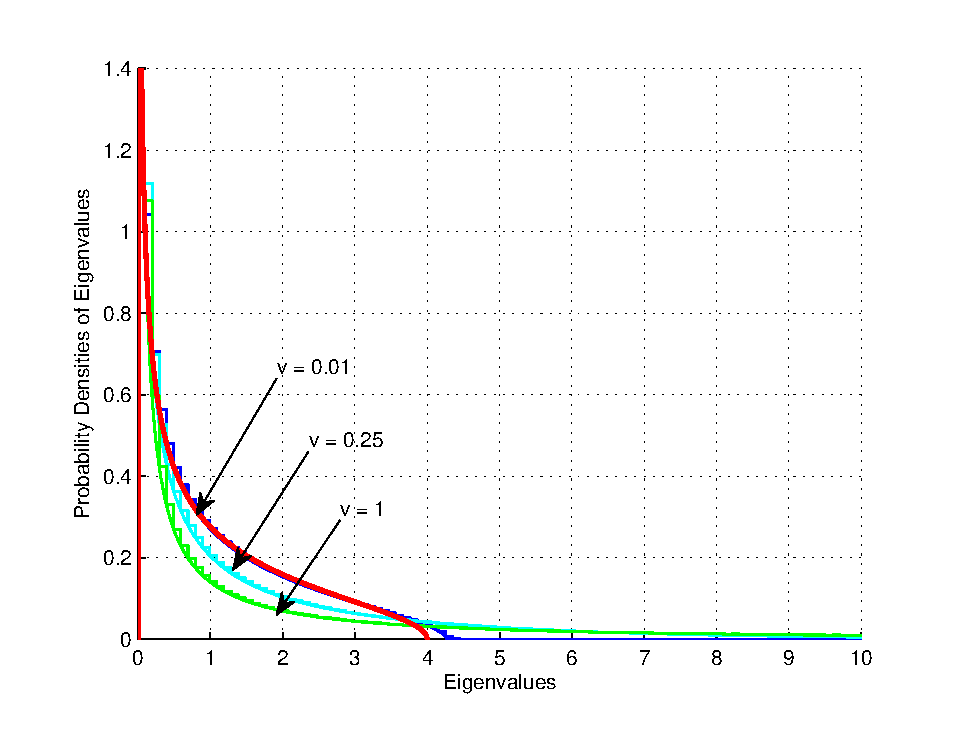
\includegraphics[scale=0.35]{../pics/Lognormal_q1.0.eps}
    \label{fig:Lognormal_q1.0}
  }
  \caption{\small \it Spectra with lognormal volatilities. The
    empirical probability density functions are plotted as stairs. The
  density function given by the Marcenko-Pastur law is plotted as a
  thick red curve.}
  \label{fig:LognormalSpectra}
\end{figure}
From figures \ref{fig:LognormalSpectra} one can see that the
Marcenko-Pastur law is recovered when $v \to 0$, as expected.

When $v$ is small, the integrands in \eqref{eq:LognormalBlueReal} and
\eqref{eq:LognormalBlueImag} have sharp maxima at $v = 0$. Hence it is
useful to approximate them by Taylor expansion. Let's write
\begin{eqnarray*}
  \lambda &=& \int _{-\infty }^{\infty }\!g \left( s,v \right) F \left( s
  \right) {ds}+{\frac {x}{{x}^{2}+{y}^{2}}} \\
  0 &=& \int _{-\infty }^{\infty }\!g \left( s,v \right) G \left( s
  \right) {ds}-{\frac {y}{{x}^{2}+{y}^{2}}}
\end{eqnarray*}
where
\begin{eqnarray*}
g &=& \frac{1}{\sqrt{2\mathop{\rm  }\pi \mathop{\rm  }v }}e^{-\frac{s
    ^{2}}{2\mathop{\rm  }v }}\\
F \left(s \right) &=& \frac{\left(e^{-2\mathop{\rm  }s }-q \mathop{\rm
    }x \right)}{\left(e^{-2\mathop{\rm  }s }-q \mathop{\rm  }x
  \right)^{2}+q ^{2}\mathop{\rm  }y ^{2}}\mathop{\rm  } \\
G(s) &=& \frac{q \mathop{\rm  }y }{\left(e^{-2\mathop{\rm  }s }-q
    \mathop{\rm  }x \right)^{2}+q ^{2}\mathop{\rm  }y ^{2}}\\
\end{eqnarray*}

Taylor-expanding $F(s)$ and $G(s)$ to 2nd order in $s$ and plugging
them into \eqref{eq:LognormalBlueReal} and
\eqref{eq:LognormalBlueImag} gives
\begin{eqnarray}
\lambda &=& {-q x+1 \over (-q x+1)^2+q^2 y^2} + {v \over 2}\left\{
{4 \over (-q x+1)^2+q^2 y^2} -{24 (-q x+1) \over
  [(-q x+1)^2+q^2 y^2]^2} \right. \nonumber \\
&& \left. + {32 (-q x+1)^3 \over [(-q x+1)^2+q^2 y^2]^3} -8 {(-q
    x+1)^2 \over [(-q x+1)^2+q^2 y^2]^2}
\right\} \label{eq:lambda_linear}\\
0 &=& {q y \over (-q x+1)^2+q^2 y^2} + {v \over 2} \left\{
  {32 q y (-q x+1)^2 \over [(-q x+1)^2+q^2 y^2]^3}
  -{8 q y \over [(-q x+1)^2+q^2 y^2]^2} \right. \nonumber \\
  && \left.
    -{8 q y (-q x+1) \over [(-q x+1)^2+q^2 y^2]^2}
\right\} \label{eq:constraint_linear}
\end{eqnarray}
Now that we look for a solution in the limit $y \to 0$, we set $y = 0$
in \eqref{eq:lambda_linear}; in \eqref{eq:constraint_linear} we first
cancel the factor $y$ and then set $y = 0$. This yields
\begin{eqnarray}
  \lambda &=& {1 \over (-q x+1)} + {2 v (q x+1) \over (-q x+1)^3} + {1
    \over x} \label{eq:lambda_1} \\
  0 &=& {q \over (-q x+1)^2} + {4 v q(q x+2) \over (-q x+1)^4} - {1
    \over x^2} \label{eq:constraint_1}
\end{eqnarray}
Evaluating \eqref{eq:lambda_1} at $x = \lambda^{MP}_{+} = (1 +
\sqrt{q})^2$ gives a rough estimate about the expected maximum
eigenvalue, respectively. That is
\begin{eqnarray}
  \lambda_{+} &=& \lambda_{+}^{MP} [1+2v(2\sqrt q +
  1)] \label{eq:lambda_3}
\end{eqnarray}
This result is checked against simulations, as shown in figure
\ref{fig:lambda_verified}. Clearly one can see that the linear
approximation \eqref{eq:lambda_3} fits fairly well to the estimated
$\E \lambda_\M$.
\begin{figure}[htb!]
  \centering
  \subfigure[$q = 0.1$]{
    \includegraphics[scale=0.35]{../pics/lambda_max_q0.1.eps}
    \label{fig:lambda_max_q0.1}
  }
  \subfigure[$q = 0.2$]{
    \includegraphics[scale=0.35]{../pics/lambda_max.eps}
    \label{fig:lambda_max_q0.2}
  }
  \subfigure[$q = 0.5$]{
    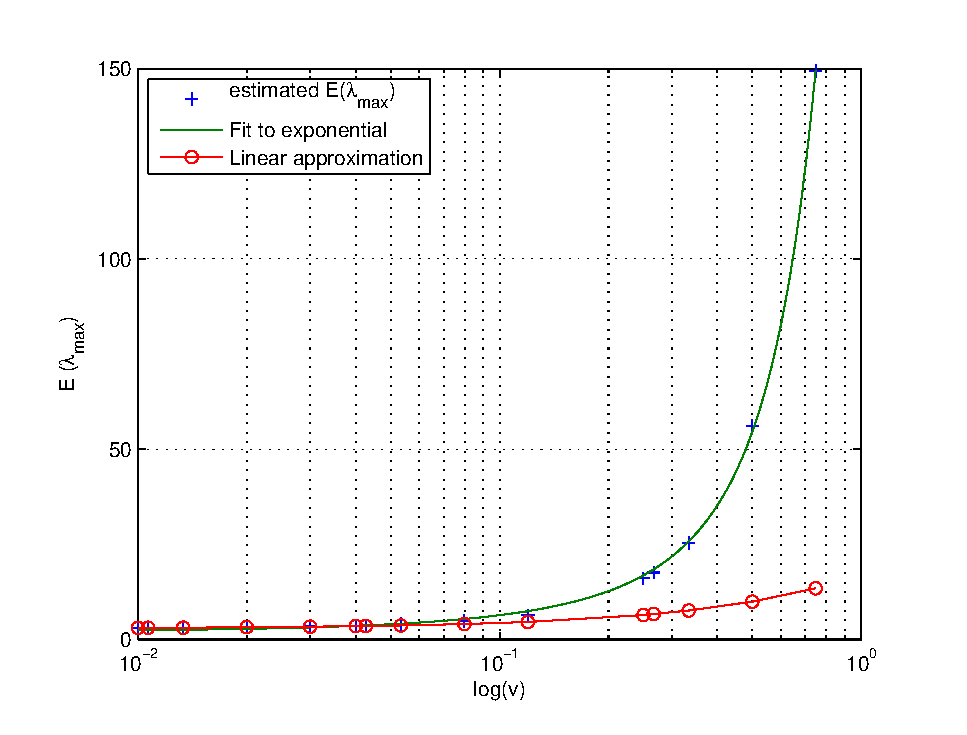
\includegraphics[scale=0.35]{../pics/lambda_max_q0.5.eps}
    \label{fig:lambda_max_q0.5}
  }
  \subfigure[$q = 1.0$]{
    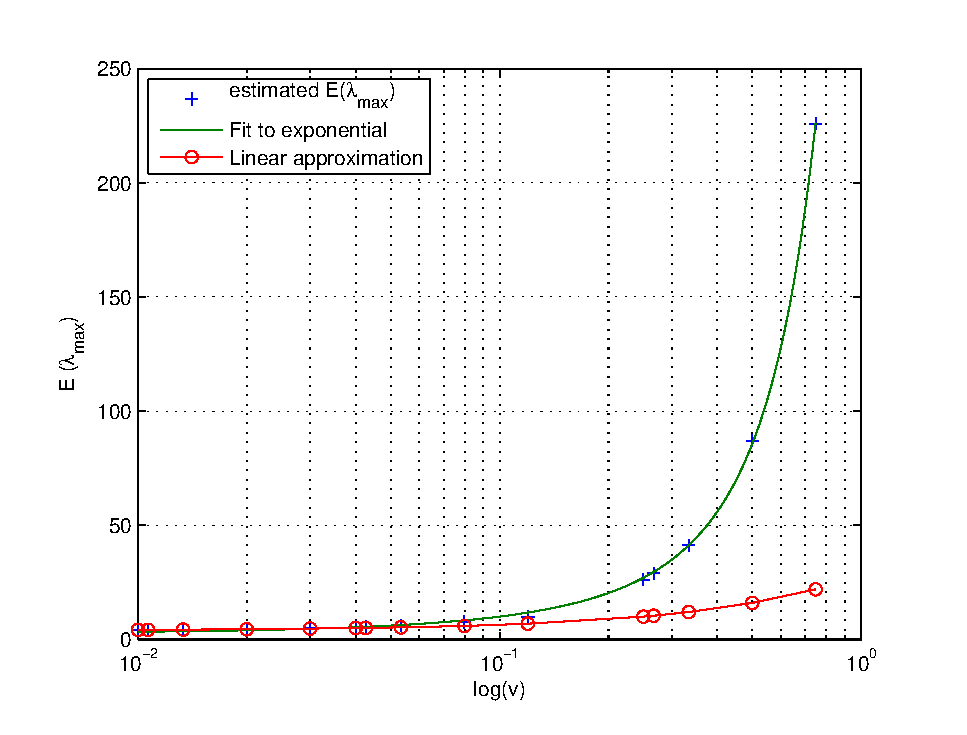
\includegraphics[scale=0.35]{../pics/lambda_max_q1.0.eps}
    \label{fig:lambda_max_q1.0}
  }
  \caption{\small \it Estimated $\E \lambda_\M$ against its linear
    approximation.}
  \label{fig:lambda_verified}
\end{figure}

\bibliographystyle{unsrt}
\bibliography{econophysics}
\end{document}
